\documentclass[a4paper]{article}
\usepackage[utf8]{inputenc}
\usepackage[russian]{babel}
\usepackage[T2]{fontenc}
\usepackage[warn]{mathtext}
\usepackage{graphicx}
\usepackage{amsmath}
\usepackage{floatflt}
\usepackage[left=20mm, top=20mm, right=20mm, bottom=20mm, footskip=10mm]{geometry}
\usepackage{capt-of}
\usepackage{pgfplots,tikz,circuitikz}
\usepackage{pgfplotstable}
\usepackage{tkz-euclide}


\graphicspath{ {images/} }
\usepackage{multicol}
\setlength{\columnsep}{2cm}


\begin{document}

\begin{titlepage}
	\centering
	\vspace{5cm}
	{\scshape\LARGE Московский физико-технический институт \par}
	\vspace{4cm}
	{\scshape\Large Лабораторная работа 3.3.6 \par}
	\vspace{1cm}
	{\huge\bfseries Влияние магнитного поля на проводимость полупроводников \par}
	\vspace{1cm}
	\vfill
\begin{flushright}
	{\large выполнил студент 924 группы ФОПФ}\par
	\vspace{0.3cm}
	{\LARGE Панферов Андрей}
\end{flushright}
	

	\vfill

% Bottom of the page
	Долгопрудный, 2020 г.
\end{titlepage}

\textbf{Цель работы:} Измерение зависомости сопротивления полупроводников от магнитного поля в них.\\

\textbf{В работе используются:} стабилизированный источник постоянного тока и напряжения, электромагнит, цифровой вольтметр, aмперметр, миллиамперметр, реостат, измеритель магнитной индукции III1-10, образцы (InSb) монокристаллического антимонида индия n-типа.\\

\textbf{Экспериментальная установка:} Схема установки для исследования магнетосопротивления полупроводников и геометрического резистивного эффекта представлена на рис. 1.

\begin{figure}[h]
    \centering
    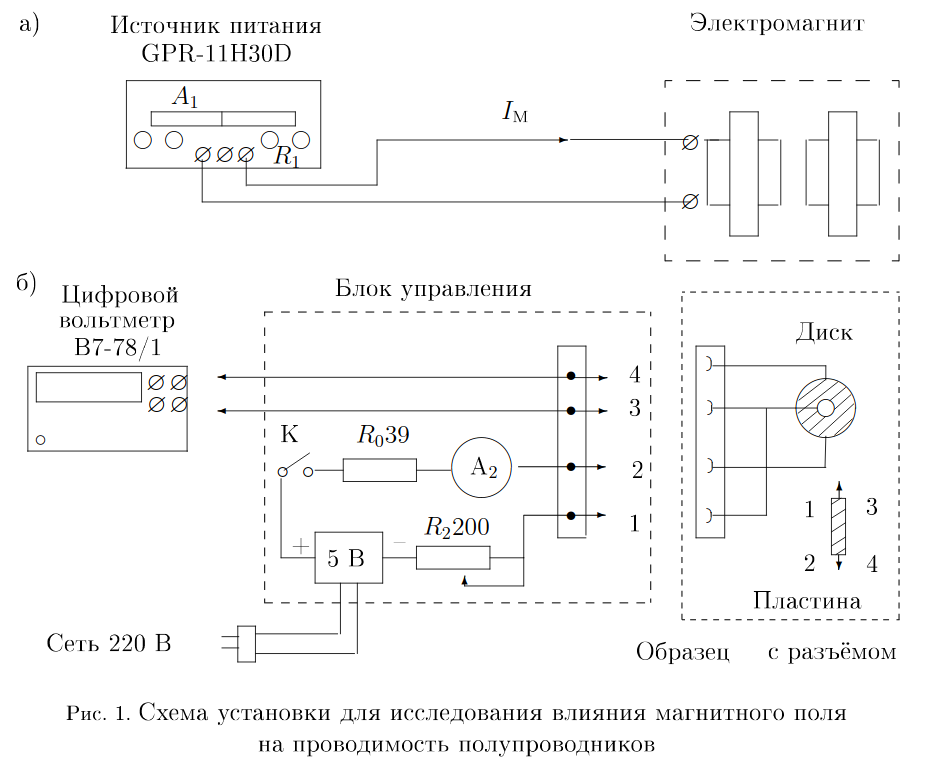
\includegraphics[width=0.8\textwidth]{scheme.png}
\end{figure}

В зазоре электромагнита создаётся постоянное магнитное поле. Ток питания магнита подаётся от источника постоянного напряжения GPR-11H30D, регулируется ручками управления источника $\left(R_{1}\right)$ и измеряется амперметром источника $A_{1}$. Магнитная индукция в зазоре электромагнита определяется при помощи измерителя магнитной индукции Ш1-10 (описание прибора расположено на установке).

Образец в форме кольца (диск Корбйно) или пластинки, смонтирован-
ный в специальном держателе, подключается к источнику постоянного напряжения 5 В. При замыкании ключа К сквозь образец течёт ток, величина которого измеряется миллиамперметром $A_{2}$ и регулируется реостатом $R_{2}$ Балластное сопротивление $R_{0}$ ограничивает ток через образец. Измеряемое напряжение подаётся на вход цифрового вольтметра $\mathrm{B} 7-78 / 1$

\newpage

\section{Калибровка магнита}

\begin{table}[ht]
\begin{minipage}{0.3\textwidth}
    \centering
    \begin{tabular}{|l|l|}
        \hline
        $I$, mA           & $B$, mT           \\ \hline
        0                 & 12                \\ \hline
        50                & 81                \\ \hline
        100               & 144               \\ \hline
        150               & 197               \\ \hline
        200               & 248               \\ \hline
        250               & 304               \\ \hline
        300               & 338               \\ \hline
        350               & 360               \\ \hline
        390               & 370               \\ \hline
        $\sigma I$ = 10mA & $\delta B$ = 0.01 \\ \hline
    \end{tabular}
    \label{table::magnet}
    \caption{Калибровка магнита}
\end{minipage}
\begin{minipage}{0.3\textwidth}
    Измерим зависимость напряженности магнитного поля в зазоре электромагнита от тока через него. Занесем результаты в \textit{Таблицу \ref{table::magnet}}. Построим \textit{График \ref{plot::magnet}} зависимости $B(I_M)$:\\
\end{minipage}
\begin{minipage}{0.5\textwidth}
    \begin{tikzpicture}[scale=0.8]
    	\begin{axis}[
    		axis lines = left,
        	xlabel = {$I$, mA},
        	ylabel = {$B$, mT},
        	ylabel style={red, scale=1},
        	xlabel style={red, scale=1},
        	%xmin=0, xmax=9,
        	title={Зависимость $B(I_M)$},
        	legend style={at={(0.03,-0.4)},anchor=west}
    		]
    		\addplot +[blue, only marks]  plot[
			error bars/.cd,
			x dir = both,
			x fixed = 10,
			y dir = both,
			y fixed relative=0.01,
		    ]
		    table[x=I, y=B, col sep=semicolon]{mag.csv};
    	\end{axis}
    	\label{plot::magnet}
    \end{tikzpicture}
\end{minipage}
\end{table}


\section{Результаты измерений}
\subsection{Диск Корбино}

\begin{table}[ht]
\begin{minipage}{0.7\textwidth}
    \centering
    \begin{tabular}{|l|l|l|l|l|}
    \hline
    $U$, mV    & $I$, mA  & $U_{down}$,  mV & $B^2$,  m(T)$^2$ & $R$, Ом \\ \hline
    779        & Без поля &                 &                  &         \\ \hline
    783        & 0        & 782             & 0.1              & 31.3    \\ \hline
    920        & 50       & 917             & 6.6              & 36.8    \\ \hline
    1280       & 100      & 1245            & 20.7             & 51.2    \\ \hline
    1724       & 150      & 1744            & 38.8             & 69      \\ \hline
    2367       & 200      & 2357            & 61.5             & 94.7    \\ \hline
    2950       & 250      & 2985            & 92.4             & 118     \\ \hline
    3338       & 300      & 3395            & 114.2            & 133.5   \\ \hline
    3608       & 350      & 3616            & 129.6            & 144.3   \\ \hline
    3818       & 400      & 3797            & 136.9            & 152.7   \\ \hline
    Параметры: & \multicolumn{4}{l|}{$D$ = 18mm, $d$ = 3mm, $H$ = 1.8mm} \\ \hline
    \end{tabular}
    \label{table::ring}
    \caption{Диск Корбино}
\end{minipage}
\begin{minipage}{0.3\textwidth}
    Измерим зависимость напряжения на образце от тока через электромагнит. Занесем результаты в \textit{Таблицу \ref{table::ring}}. Расчитаем сопротивления образца и квадраты величин напряженности магнитного поля. Также занесем в таблицу размеры образца.
\end{minipage}
\end{table}

\subsection{Параллелепипед}

\begin{table}[ht]
\begin{minipage}{0.7\textwidth}
    \centering
    \begin{tabular}{|l|l|l|l|l|l|}
    \hline
    $U$, mV & $I$, mA  & $U_{\perp}$,  mV & $B^2$,  m(T)$^2$ & $R$, Ом & $R_{\perp}$, Ом \\ \hline
    2775    & Без поля &                  &                  &         &                 \\ \hline
    2759    & 0        & 2758             & 0.1              & 275.9   & 275.8           \\ \hline
    2818    & 50       & 2803             & 6.6              & 281.8   & 280.3           \\ \hline
    2904    & 100      & 2888             & 20.7             & 290.4   & 288.8           \\ \hline
    3035    & 150      & 2968             & 38.8             & 303.5   & 296.8           \\ \hline
    3177    & 200      & 3063             & 61.5             & 317.7   & 306.3           \\ \hline
    3283    & 250      & 3158             & 92.4             & 328.3   & 315.8           \\ \hline
    3370    & 300      & 3213             & 114.2            & 337     & 321.3           \\ \hline
    3427    & 350      & 3276             & 129.6            & 342.7   & 327.6           \\ \hline
    3454    & 400      & 3454             & 136.9            & 345.4   & 345.4           \\ \hline
    \end{tabular}
    \label{table::par}
    \caption{Параллелепипед}
\end{minipage}
\begin{minipage}{0.3\textwidth}
    Измерим зависимость напряжения на образце от тока через электромагнит. Занесем результаты в \textit{Таблицу \ref{table::par}}. Расчитаем сопротивления образца для обеих положений и квадраты величин напряженности магнитного поля.
\end{minipage}
\end{table}

\section{Обработка данных}

\begin{minipage}{0.5\textwidth}
    \begin{tikzpicture}[scale=1]
    	\begin{axis}[
    		axis lines = left,
        	xlabel = {$B^2$, m(T$^2$)},
        	ylabel = {$R$, Ом},
        	ylabel style={red, scale=1},
        	xlabel style={red, scale=1},
        	xmin=0, ymin=0,%xmax=9,
        	title={Зависимость $R(B^2)$},
        	legend style={at={(0.03,-0.4)},anchor=west, scale=0.7}
    		]
    		\addplot +[blue, only marks]  plot[
			error bars/.cd,
			x dir = both,
			x explicit,
			y dir = both,
			y fixed relative=0.004,
		    ]
		    table[x=B2, x error=DB2, y=RR, col sep=semicolon]{MegaPlot.csv};
		    \addlegendentry{Диск Корбино};
		    \addplot +[red, only marks]  plot[
			error bars/.cd,
			x dir = both,
			x explicit,
			y dir = both,
			y fixed relative=0.01,
		    ]
		    table[x=B2, x error=DB2, y=R, col sep=semicolon]{MegaPlot.csv};
		    \addlegendentry{Параллелепипед};
		    \addplot +[green, only marks]  plot[
			error bars/.cd,
			x dir = both,
			x explicit,
			y dir = both,
			y fixed relative=0.01,
		    ]
		    table[x=B2, x error=DB2, y=RP, col sep=semicolon]{MegaPlot.csv};
		    \addlegendentry{Параллелепипед перпендикулярно};
		    \addplot [color=blue, domain=0:130]{0.8807*x + 33.59};
    	\end{axis}
    	\label{plot::mega}
    \end{tikzpicture}
\end{minipage}
\begin{minipage}{0.5\textwidth}
    Построим \textit{График \ref{plot::mega}} зависимости $R(B^2)$ для всех трех серий измерений. Из графика найдем подвижность носителей и другие параметры материала (InSb) диска Корбино, сравним с табличными:
    \begin{align*}
        \mu^2 &= \frac{dR}{d(B^2)} \\
        \mu_{InSb} &= 30 \pm 1 \:m^2/(V \cdot s) \\
        \mu_{tab} &= 7.7 \:m^2/(V \cdot s) \\
        \sigma_0 &= \frac{1}{2\pi h R_0} ln\frac{r_2}{r_1} = (0.517 \pm 0.007) \: 1/(Om \cdot m) \\
        \sigma_{tab} &= 2.2\cdot10^4 \: 1/(Om \cdot m)\\
        n &= \frac{\sigma}{q\mu} = (1.07 \pm 0.04)\cdot 10^{17} 1/m^3 \\
        n_{tab} &= 1.78 \cdot 10^{22} 1/m^3\\
    \end{align*}
\end{minipage}

\section{Вывод}
Мы измерили концентрацию носителей заряда и их подвижность для антимонида индия. Результаты не попали даже в порядок табличных величин. У данных высокая воспроизводимость и относительно низкая погрешность, которая никак не может объяснить расхожения. Вероятно, ошибка в параметрах образца или диапазонах измерения приборов.





\end{document}
